\subsection{Pengujian Komponen \textit{Predictor}}

Pada bagian ini akan dijelaskan tentang tujuan, skenario, hasil, dan analisis dari pengujian komponen \textbf{\textit{Predictor}}.

\subsubsection{Tujuan Pengujian}

Tujuan pengujian ini memastikan komponen \textbf{\textit{Predictor}} dapat berjalan dengan baik dan menghasilkan data yang sesuai dengan ekspektasi.

\subsubsection{Skenario Pengujian}

Pengujian terhadap komponen \textbf{\textit{Predictor}} dilakukan dengan membandingkan hasil prediksi dengan aktual untuk skenario sebagai berikut.
\begin{enumerate}
    \item \textit{Elastic Search} sedang \textit{idle}.
    \item \textit{Elastic Search} sedang digunakan untuk melakukan operasi penambahan data.
    \item \textit{Elastic Search} sedang digunakan untuk melakukan operasi pencarian data.
\end{enumerate}

\subsubsection{Hasil Pengujian dan Analisis}

% \begin{figure}[h]
%     \centering
%     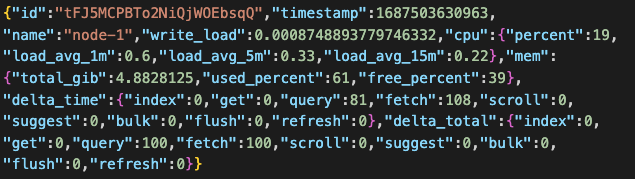
\includegraphics[width=0.8\textwidth]{chapter-4/mf-3.png}
%     \caption{Hasil Pengujian Komponen \textit{Metrics Fetcher} Skenario 3}
%     \label{fig:mf-3}
% \end{figure}

Pengujian komponen \textbf{\textit{Predictor}} menghasilkan angka yang cukup baik sehingga hasil prediksinya bisa dianggap merepresentasikan kondisi aktual.